%\documentclass[a4paper,10pt]{article}
\documentclass[times, 10pt,twocolumn]{article} 
\usepackage{latex8}
\usepackage{times}
\usepackage[dvips,pdftex]{graphicx}
%\usepackage{array}
%\usepackage[caption=false]{caption}
\usepackage[tight,footnotesize]{subfigure}

% take the % away on next line to produce the final camera-ready version 
\pagestyle{empty}
 
%opening
\title{A Novel Domain-Specific Feature Extraction Scheme For Arabic Handwritten Digits Recognition}
\author{ Sherif Abdelazeem\\
Electronics Engineering Department, American University in Cairo\\
shazeem@aucegypt.edu\\
}
\begin{document}

\maketitle

\begin{abstract}
The most crucial step for the success of any character recognition system is the extraction of good features. A wide variety of well-known universal feature sets were used in character recognition problems; such as gradient, Kirsch, and contour features. This paper argues that a domain-specific features extracted based on their ability to characterize the classes at hand in a way similar to how humans intuitively discriminate among those classes can outperform universal features set. Arabic handwritten digits recognition problem is used to prove the superiority of domain specific features over universal ones. Results show that a carefully chosen feature vector of only 35 features could outperform many universal feature sets of hundreds of features in both recognition accuracy and speed.
 \end{abstract}
\section{Introduction}
The most important step in any recognition system is the feature extraction. Any recognition system performance depends on the quality of features as it depend on the classier used to make the final classification decision \cite{Lauertrainable7}. Feature extraction attempts to capture input data properties to reduce the size of the problem from the size of the original raw data to the size of the extracted features. Thus, good features are necessary for better and faster recognition process. For a better recognition system, the feature set extracted should be most relevant for the problem at hand in the sense of minimizing the within-class pattern variability while enhancing the between-class pattern variability \cite{devijiverPRstatical}.

There is a wealth of feature extraction techniques in the literature for numeral as well as character recognition in general \cite{TrierFeature}. The input pattern is characterized by a set of N features extracted from the raw data such as moment features, transform features, gradient and curvature features, geometrical and structural based features, zoning features, etc, \cite{Shiagradient,SirkantangradientContor,visionfeatures5,hustructurecode}. Among the various feature extraction techniques, gradient features in particular have proven to be somewhat superior to other feature sets \cite{benchmarking3,liunormalizegradient}. The various feature extraction techniques available in the literature are usually universal in the sense that they can be applied to many different classification problems with different degrees of success depending on the nature of the problem at hand. The major problem with universal features is that they do not match the way by which humans identify different classes in any given problem. That is, the universal features are usually unrelated to the distinguishing features that humans use to recognize the different classes in a particular problem. 

This paper demonstrates that domain-specific features are superior to universal features both in classification accuracy and speed. The classification problem at hand is the Arabic handwritten digits recognition problem. The features extracted are based on the intrinsic properties of Arabic numerals and it is shown that they do outperform universal features which do not take into account the inherent attributes of Arabic digits. 
%The rest of the paper is organized as follows. In Section \ref{sec:section2}, a review of the Arabic handwritten digits recognition problem is given. Section \ref{sec:section3} discusses the problem-specific features extracted from the Arabic digits explaining how those features match the way humans distinguish Arabic digits. Section \ref{sec:section4} provides the experimental results which clearly reveal the superior performance of the proposed features over well known universal features in terms of classification accuracy and speed. In Section \ref{sec:section5}, concluding remarks are given.

\section{Arabic Handwritten Digits Recognition}
\label{sec:section2}
 % While recognition of handwritten Latin digits has been extensively investigated using various techniques, little work has been done on Arabic handwritten digit recognition. Al-Omari et al. \cite{indiannumerals14} used a scale-, translation-, rotation-invariant feature vector to train a probabilistic neural network (PNN). Their database was composed of 720 digits for training and 480 digits for testing written by 120 persons. They achieved 99.75\% accuracy. Said et al. \cite{EnglishArabic15} used pixel values of the normalized digit images as features. They fed these values to an Artificial Neural Network (ANN). They used a training set of 2400 digits and a testing set of 200 digits written by 20 persons to achieve 94\% accuracy. In \cite{ADBase9}, El-Sherif and Abdelazeem devised a two-stage system for recognizing Arabic digits. The first stage is an ANN fed with a short feature vector to handle easy-to-classify digits. Ambiguous digits are rejected to the more powerful second stage which is an SVM fed with a long feature vector. The system had a good timing performance and achieved 99.15\% accuracy. Note that results of different works cannot be compared because the used databases are not the same. 
Abdelazeem and El-Sherif \cite{IjdarSherifPaper} did a comprehensive study on the problem of Arabic handwritten digit recognition. They reported the performances of different classification and universal feature extraction techniques on recognizing handwritten Arabic digits. They also introduced a large binary Arabic handwritten Digits dataBase(the ADBase) and a modified gray level version of it (Modified ADBase or MADBase). Table \ref{tab:arabicandlatin} shows Arabic handwritten digits with different writing styles as well as their printed versions.
\begin{table}[h]
\begin{center}
\caption{Arabic Printed and Handwritten Digits.}
	\label{tab:arabicandlatin}
\scalebox{0.8}{
	\begin{tabular}{|l|l|l|l|l|l|l|l|l|l|l|}
	\hline
	Latin Equivalent & 0 & 1 & 2 & 3 & 4 & 5 & 6 & 7 & 8 & 9 \\ 
	\hline
	Printed & \includegraphics[scale=0.2]{images/0.JPG}  &  \includegraphics[scale=0.18] {images/1.JPG}   
	& \includegraphics[scale=0.2] {images/2.JPG} &  \includegraphics[scale=0.2] {images/3.JPG}  &\includegraphics[scale=0.2] {images/4.JPG}   & \includegraphics[scale=0.2] {images/5.JPG} 
&  \includegraphics[scale=0.2] {images/6.JPG}  & \includegraphics[scale=0.2] {images/7.JPG} 
	      & \includegraphics[scale=0.2] {images/8.JPG}   & \includegraphics[scale=0.2] {images/9.JPG}   \\ 
	\hline
	Typical Handwritten & \includegraphics[scale=0.2]{images/h0.JPG}  & \includegraphics[scale=0.3]{images/h1.JPG}   
	& \includegraphics[scale=0.2] {images/h2.JPG} &  \includegraphics[scale=0.2] {images/h3.JPG}  &\includegraphics[scale=0.2] {images/h4.JPG}   & \includegraphics[scale=0.2] {images/h5.JPG} 
&  \includegraphics[scale=0.2] {images/h6.JPG}  & \includegraphics[scale=0.2] {images/h7.JPG} 
	      & \includegraphics[scale=0.2] {images/h8.JPG}   & \includegraphics[scale=0.2] {images/h9.JPG}\\ 
	\hline
	Other Writing Style & -- & -- & -- & \includegraphics[scale=0.35] {images/h3_2.JPG}   & -- & -- & -- & -- & -- & -- \\ 
	\hline	
	\end{tabular}	
	}
\end{center}
\end{table}
 
\subsection{The ADBase }
The ADBase is composed of 70,000 digits written by 700 participants. Each participant wrote each digit (from '0' to  '9' ) ten times. The digits are of variable sizes. The database is partitioned into two sets: a training set (60,000 digits  6000 images per class) and a test set (10,000 digits 1000 images per class). Writers of the training set and the test set are exclusive. The Order of including writers in the test set is randomized to make sure that writers of the test set are not from a single institution (to ensure variability of the test set). 

\subsection{The MADBase}
The MADBase is a modified gray level version of the ADBase where each digit is confined in a 20$\times$20 box while preserving its ADBase aspect ratio. To encourage researchers to further study the problem of Arabic handwritten digits recognition, Both ADBase and MADBase have been made available online for free at http://datacenter.aucegypt.edu/shazeem/

\section{Domain-Specific Feature Extraction}
\label{sec:section3}
For every digit an attempt is made to generate features that make the digit unique among other numerals in a way similar to how the human mind intuitively distinguishes a given digit from all others. The ultimate purpose is to create a feature vector where every feature has a logical meaning related to some distinct characteristic of at least one of the numerals. The approach followed to extract features for every digit is explained as follows:

%\subsection*{Digit '0'}
\textsl{Digit '0':} The Arabic digit '0' is just a dot which can be of various peculiar shapes when written fast by the hand. Thus, it may get confused with almost all other digits (especially 1 and 5). However, the eye can easily differentiate between them because the digit '0' is clearly much smaller than any other digit as shown in Figure \ref{fig:fig1}. Therefore, some size features should be used to distinguish the digit '0' from all other digits. The height, width, and area of the bounding box of the ADBase represent three intuitive features for that purpose. Let the three features be denoted by 'Height\_0', 'Width\_0', 'Area\_0', respectively. 

\begin{figure}[t]
 \begin{center}
 \centering
 \subfigure[\small Arabic Digit 0]{\label{fig:fig1a}
\includegraphics[width=0.08\textwidth]{figures/fig1a.jpg}}
 \subfigure[\small Arabic Digit 1]{\label{fig:fig1b} 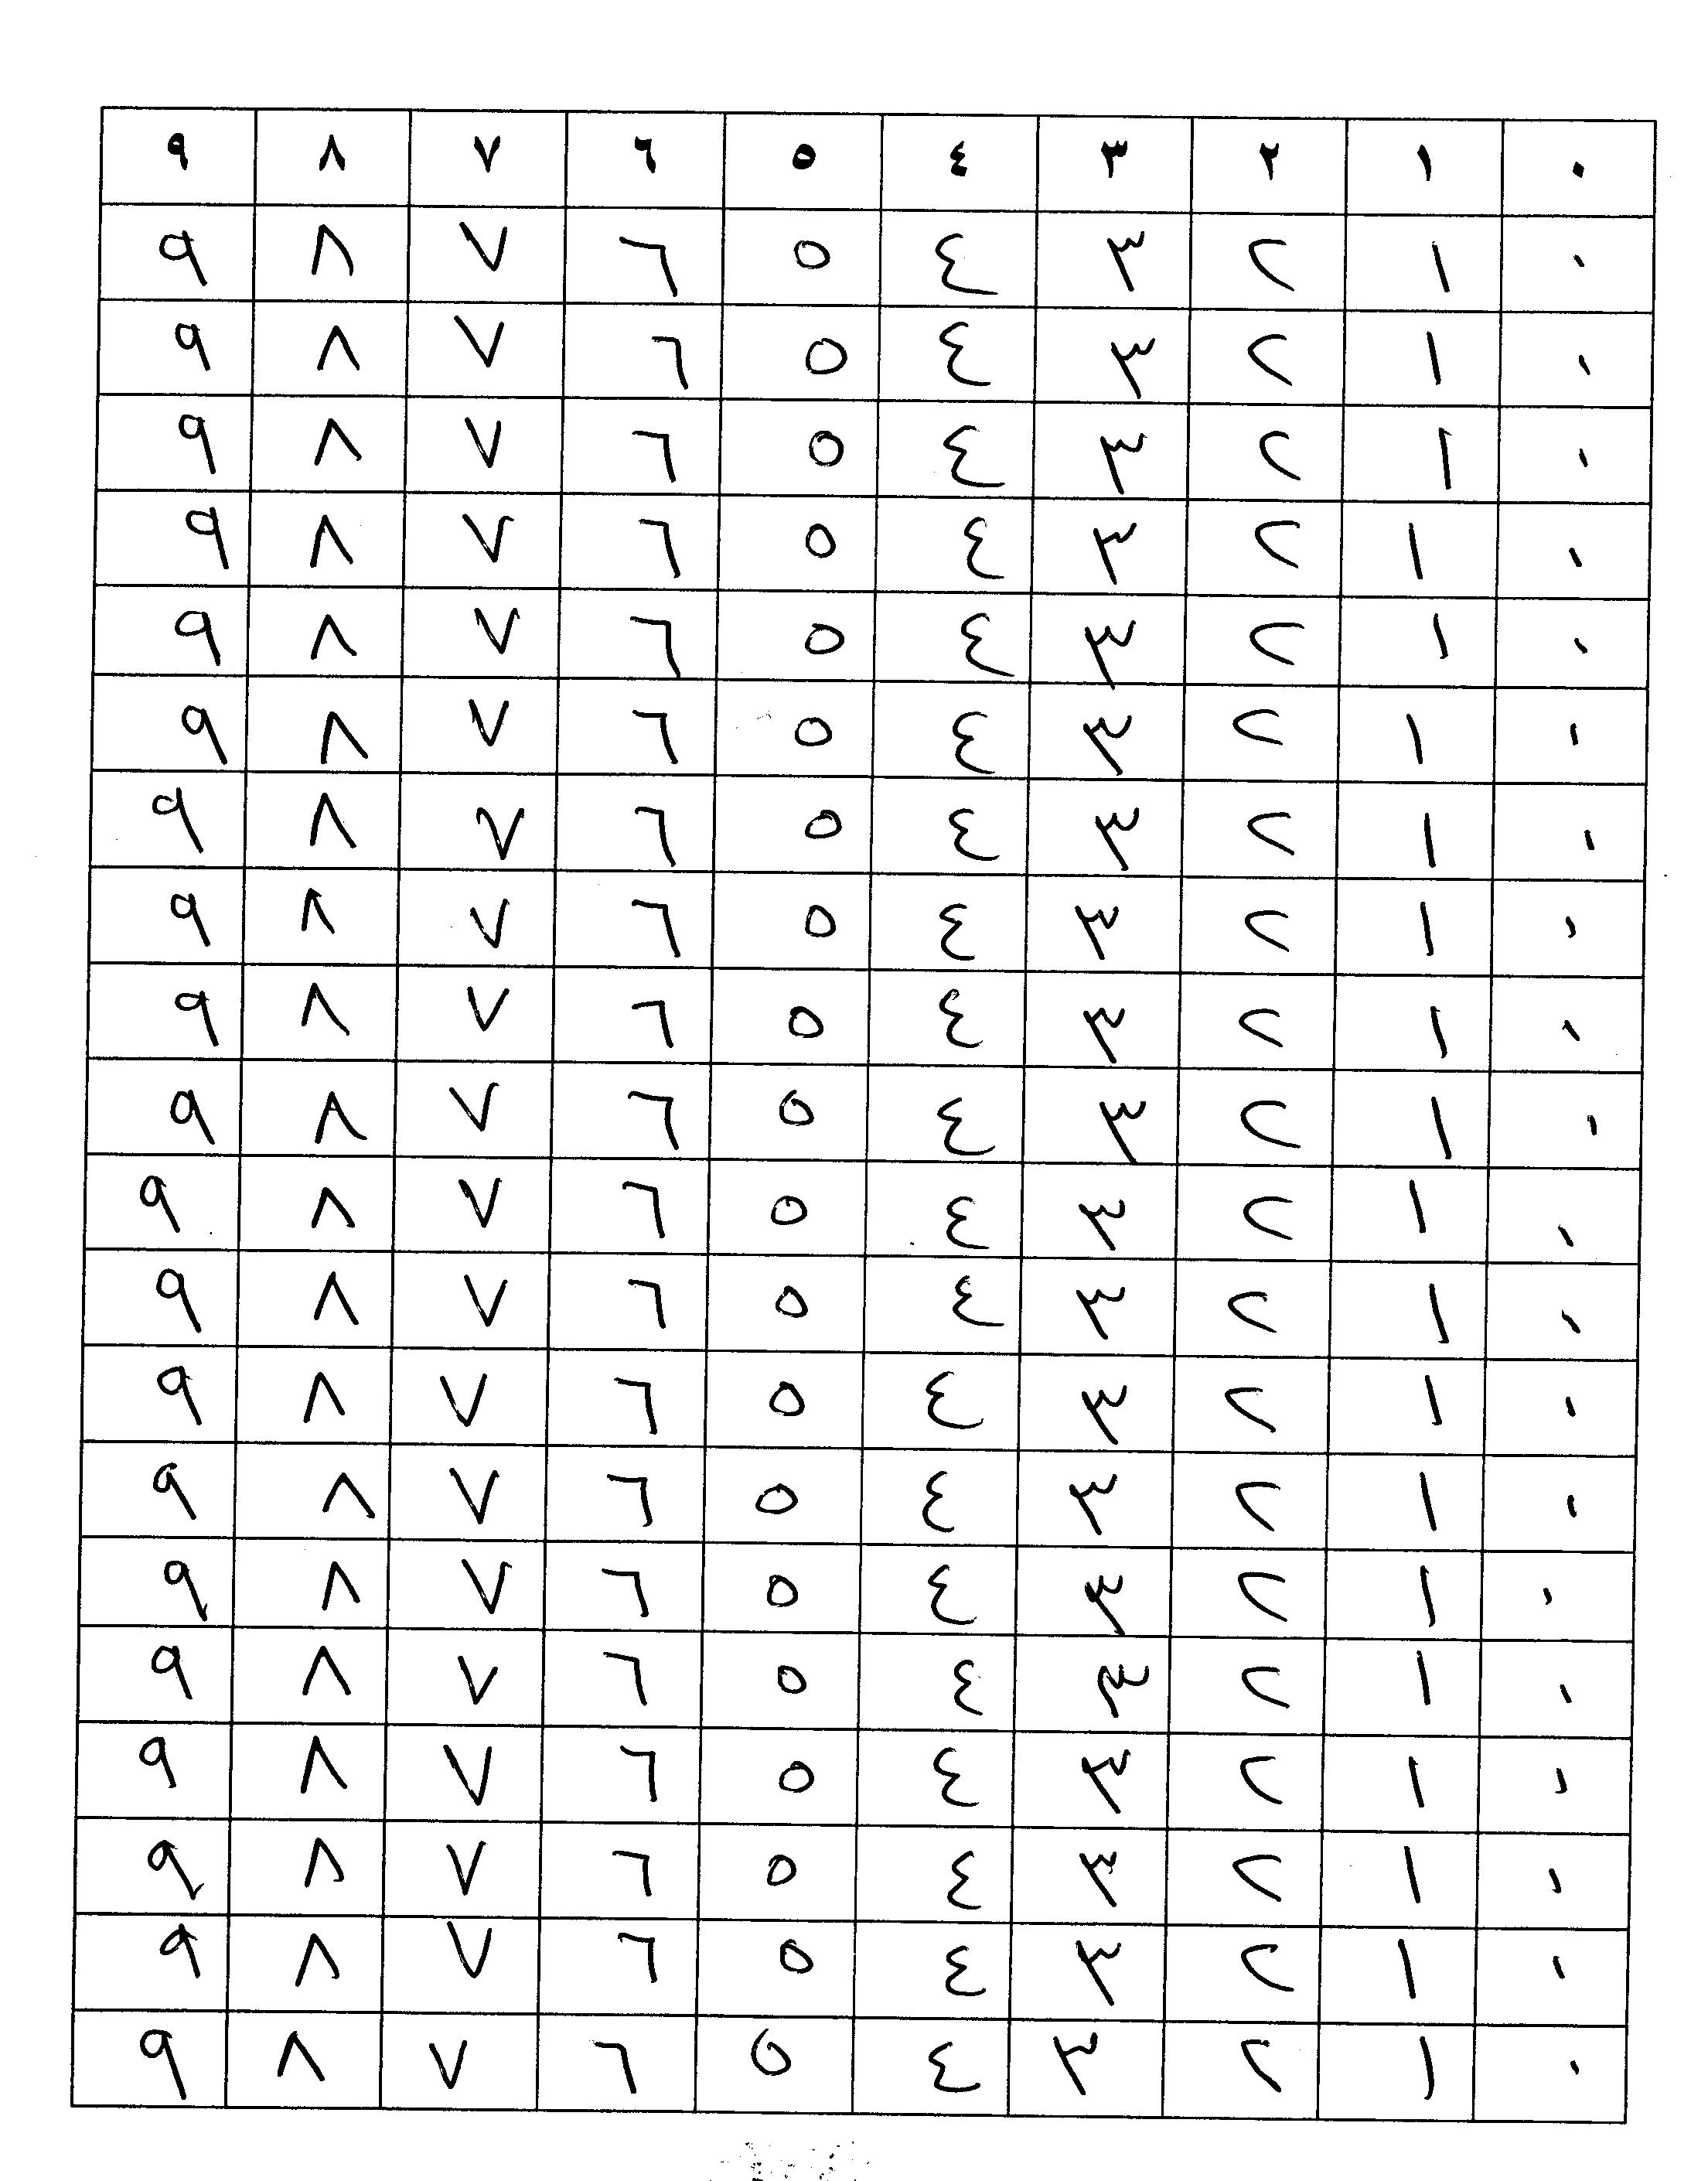
\includegraphics[width=0.08\textwidth]{figures/fig1b.jpg}}
 %\includegraphics[width=0.2\textwidth]{figures/fig1.jpg}
 % fig1.jpg.eps: 159x114 pixel, 72dpi, 5.61x4.02 cm, bb=0 0 159 114
\end{center}
\caption{Size of digit 0 with respect to digit 1.}
\label{fig:fig1}
\end{figure} 
%\subsection*{Digit '1'}

\textsl{Digit '1':} The Arabic digit '1' is easily distinguishable to the human eye by its long height compared to its short width as shown in Figure \ref{fig:fig1}. The ratio of the height to the width of the bounding box is an intuitive feature to be added to the feature set. Let the feature be denoted by 'HW\_ratio\_1'.
%\subsection*{Digit '2'}
%Figure 3.  
\begin{figure}[h]
\centering
 \subfigure[\small Feature 'White\_2'.]{\label{fig:fig3}
 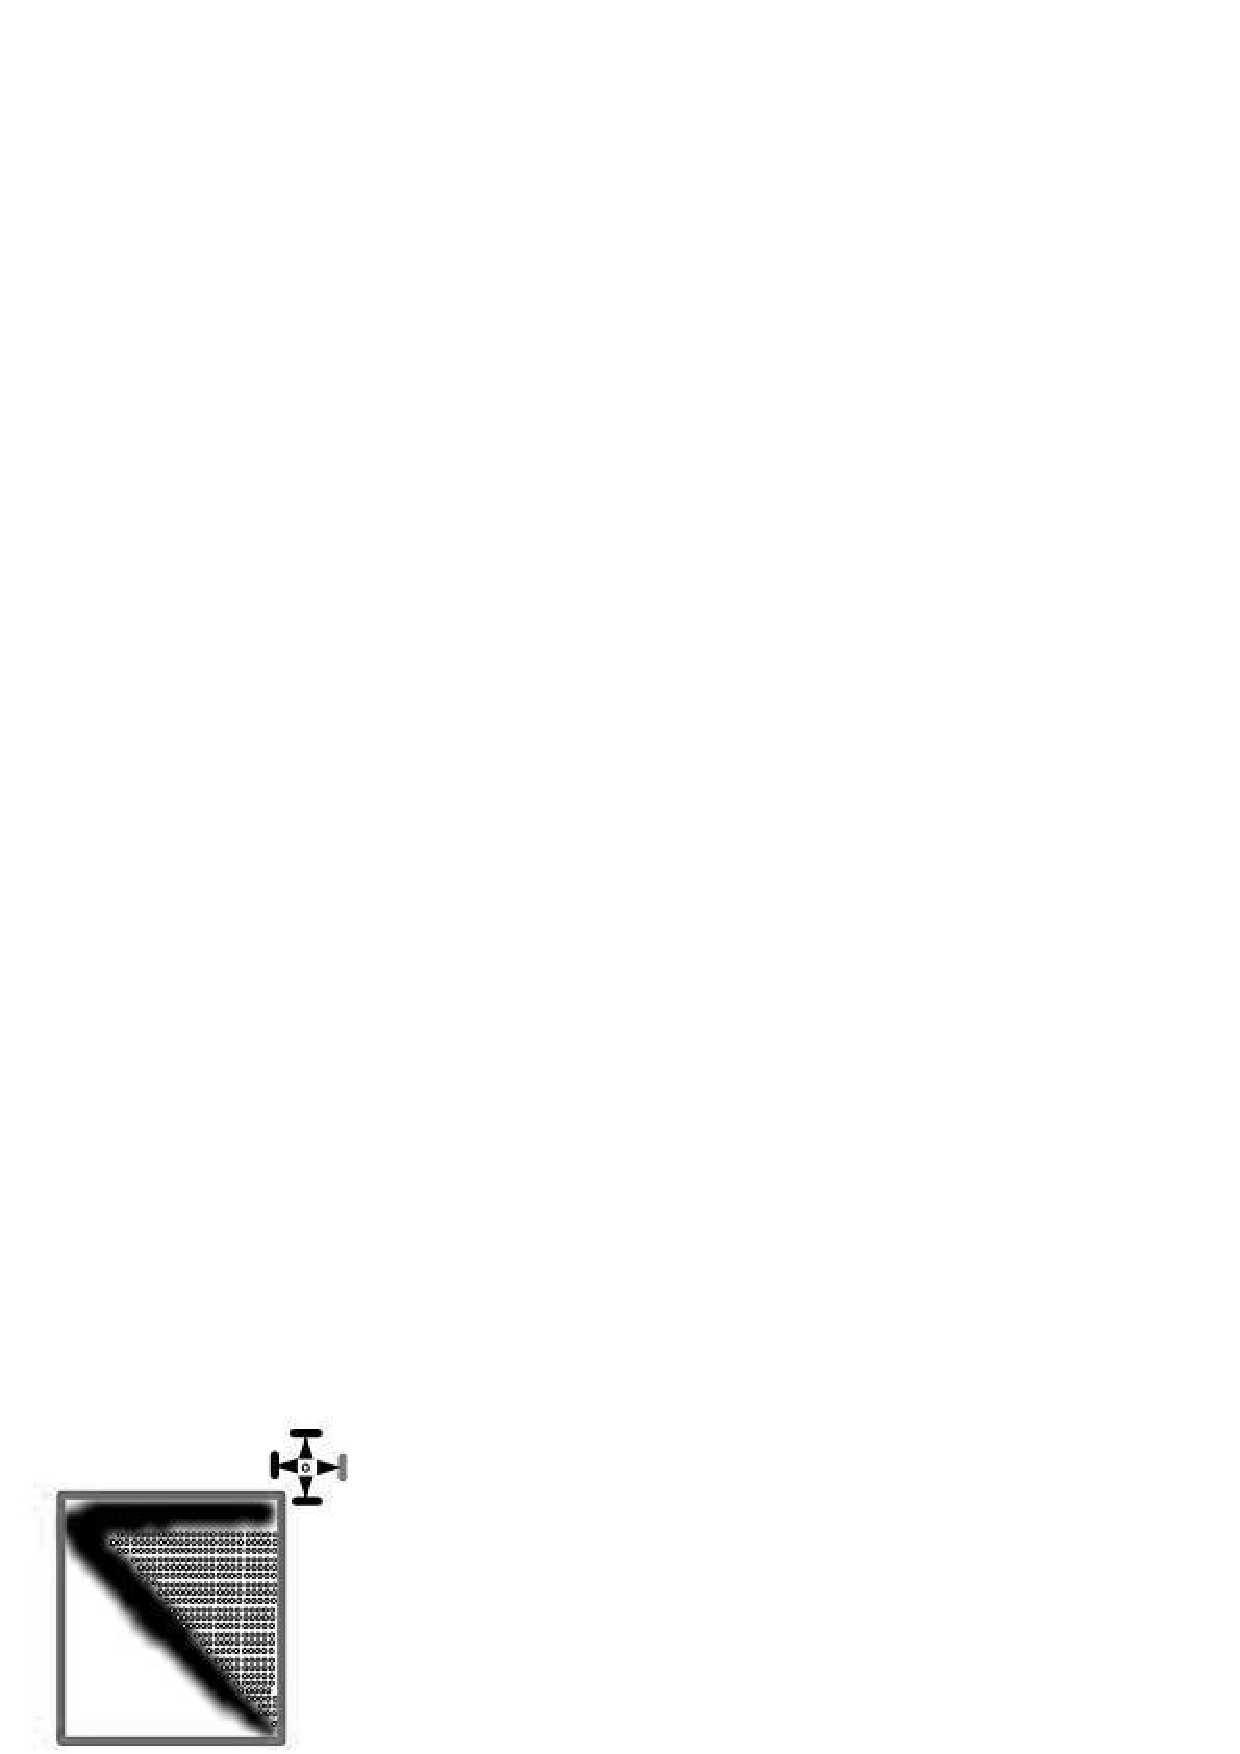
\includegraphics[width=0.12\textwidth]{figures/fig3.jpg}}
 \subfigure[\small{Feature 'White\_3'.}]{\label{fig:fig4} 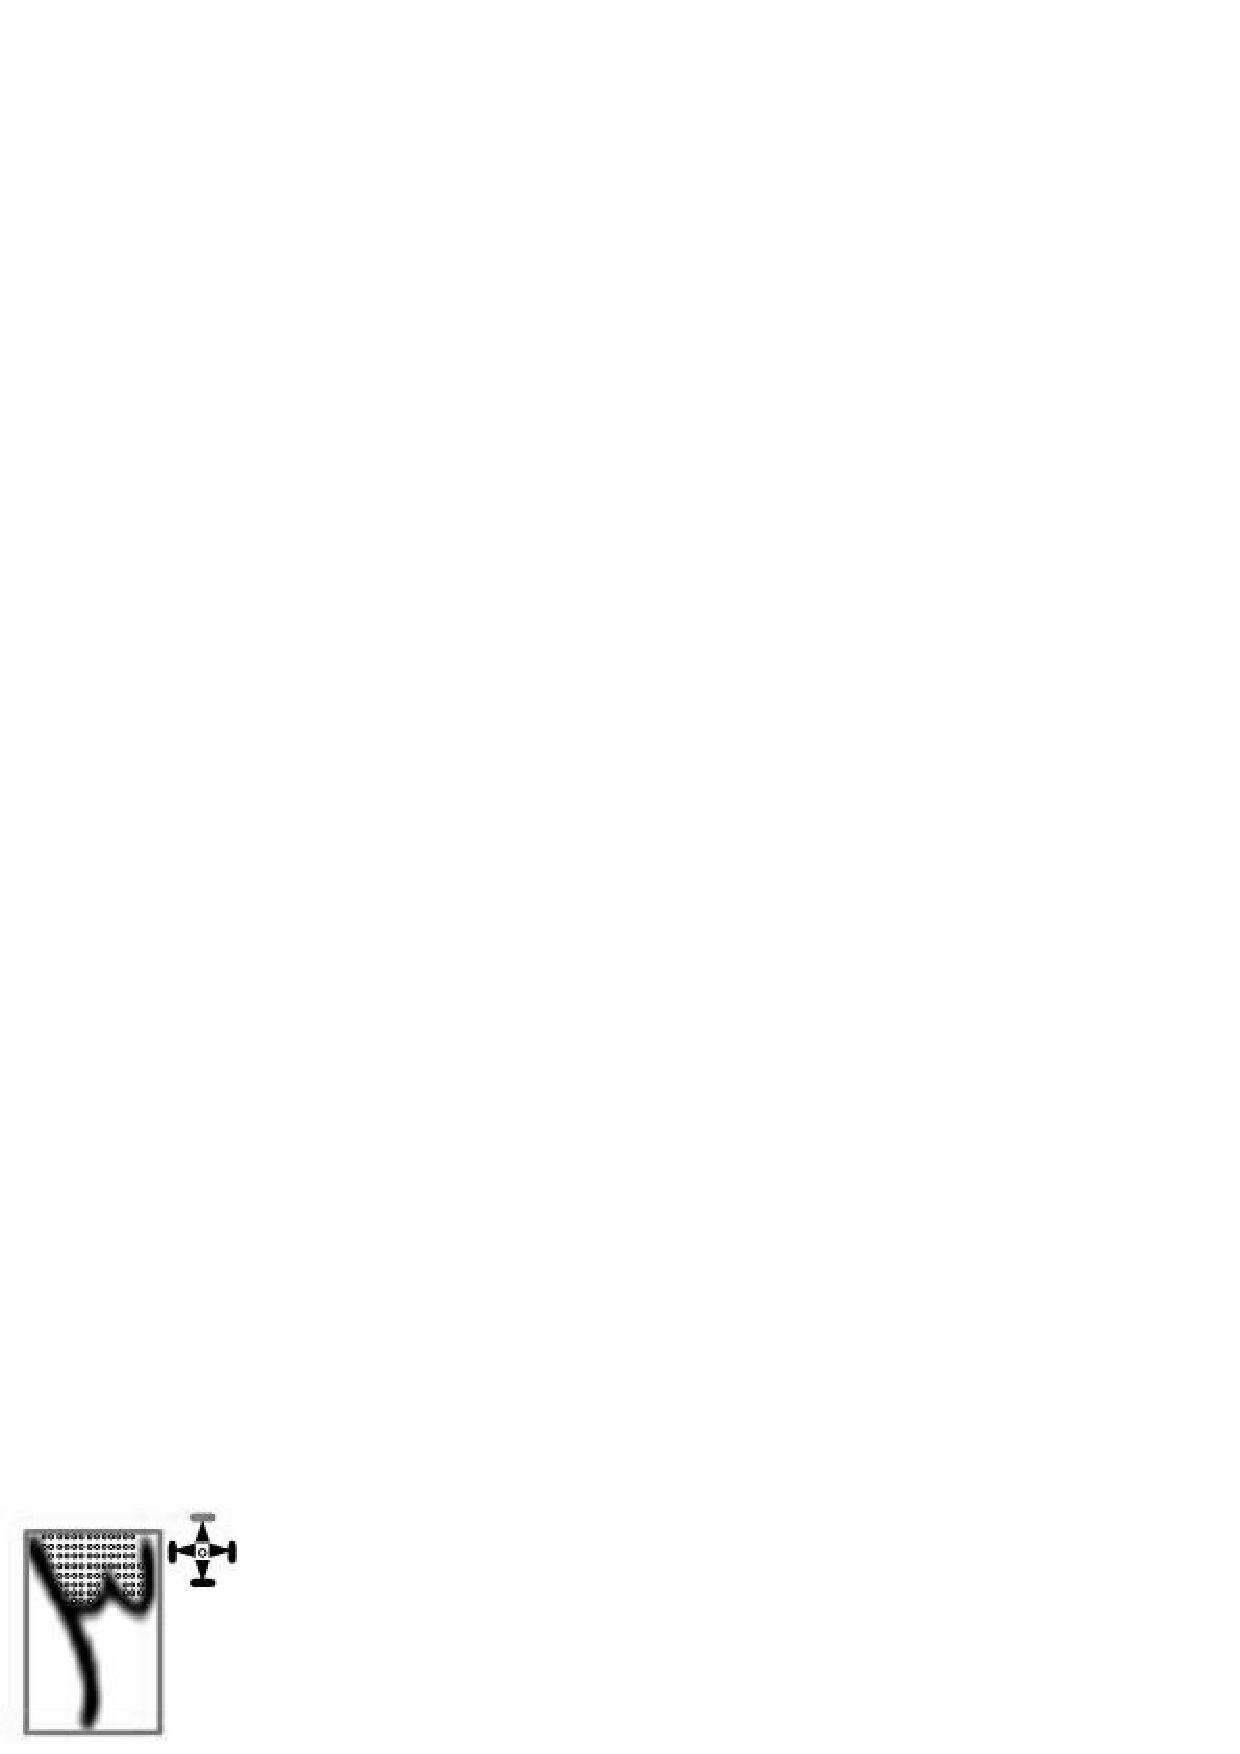
\includegraphics[width=0.13\textwidth]{figures/fig4.jpg}}
\caption{Feature 'White\_2' in Arabic Digit 2 and Feature 'White\_3' in Arabic digit 3.}
\end{figure} 

\textsl{Digit '2':} The Arabic digit '2' can be distinguished from other digits by the fact that most of the white pixels in a bounding box containing the digit '2' are confined between the right border and three black pixels from the top, the bottom and the left as shown in Figure \ref{fig:fig3}. The count of these white pixels represents an intuitive feature for Arabic digit '2'. Let the feature be denoted by 'White\_2'.
 
\textsl{Digit '3':} The Arabic digit '3' is similar in appearance to Arabic digit '2'. Thus, the same feature 'White\_2' can be used to distinguish digit '3' from other Arabic digits except digit '2'. The intuitive feature that distinguishes the digit '3' from the digit '2' is the presence of white pixels confined by the top border and black pixels from left and right. as shown in Figure \ref{fig:fig4}. The count of these white pixels represents an important intuitive feature for the digit '3' and let it be denoted by 'White\_3'.

\textsl{Digit '4':} The Arabic digit '4' has a distinct bend on its left profile. Thus, there are white pixels surrounded by black pixels from above and below and having the left corner of the bounding box to their left as clear in Figure \ref{fig:fig5}. The count of those white pixels should be added to distinguish digit '4' from all other digits and let it be denoted by 'White\_4'.
\begin{figure}
\centering
 \begin{center}
 \subfigure[Feature 'White\_4'.]{\label{fig:fig5}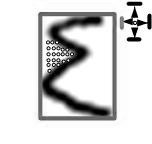
\includegraphics[width=0.15\textwidth]{figures/fig5.jpg}}
  \subfigure[Feature 'White\_5'.]{\label{fig:fig6}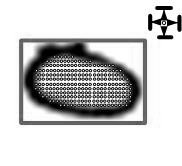
\includegraphics[width=0.15\textwidth]{figures/fig6.jpg}}
\end{center}
\caption{Feature 'White\_4' in Arabic digit 4 and feature 'White\_5' in Arabic digit 5.}
\end{figure} 

\textsl{Digit '5':} The distinguishing feature of Arabic digit '5' is that its white pixels are mainly surrounded by black pixels in all directions: top, bottom, right, and left as clear in Figure \ref{fig:fig6}. The count of these white pixels is considered one feature and denoted by 'White\_5'.
\begin{figure}
 \begin{center}
 \subfigure[Feature 'White\_6'.]{\label{fig:fig7}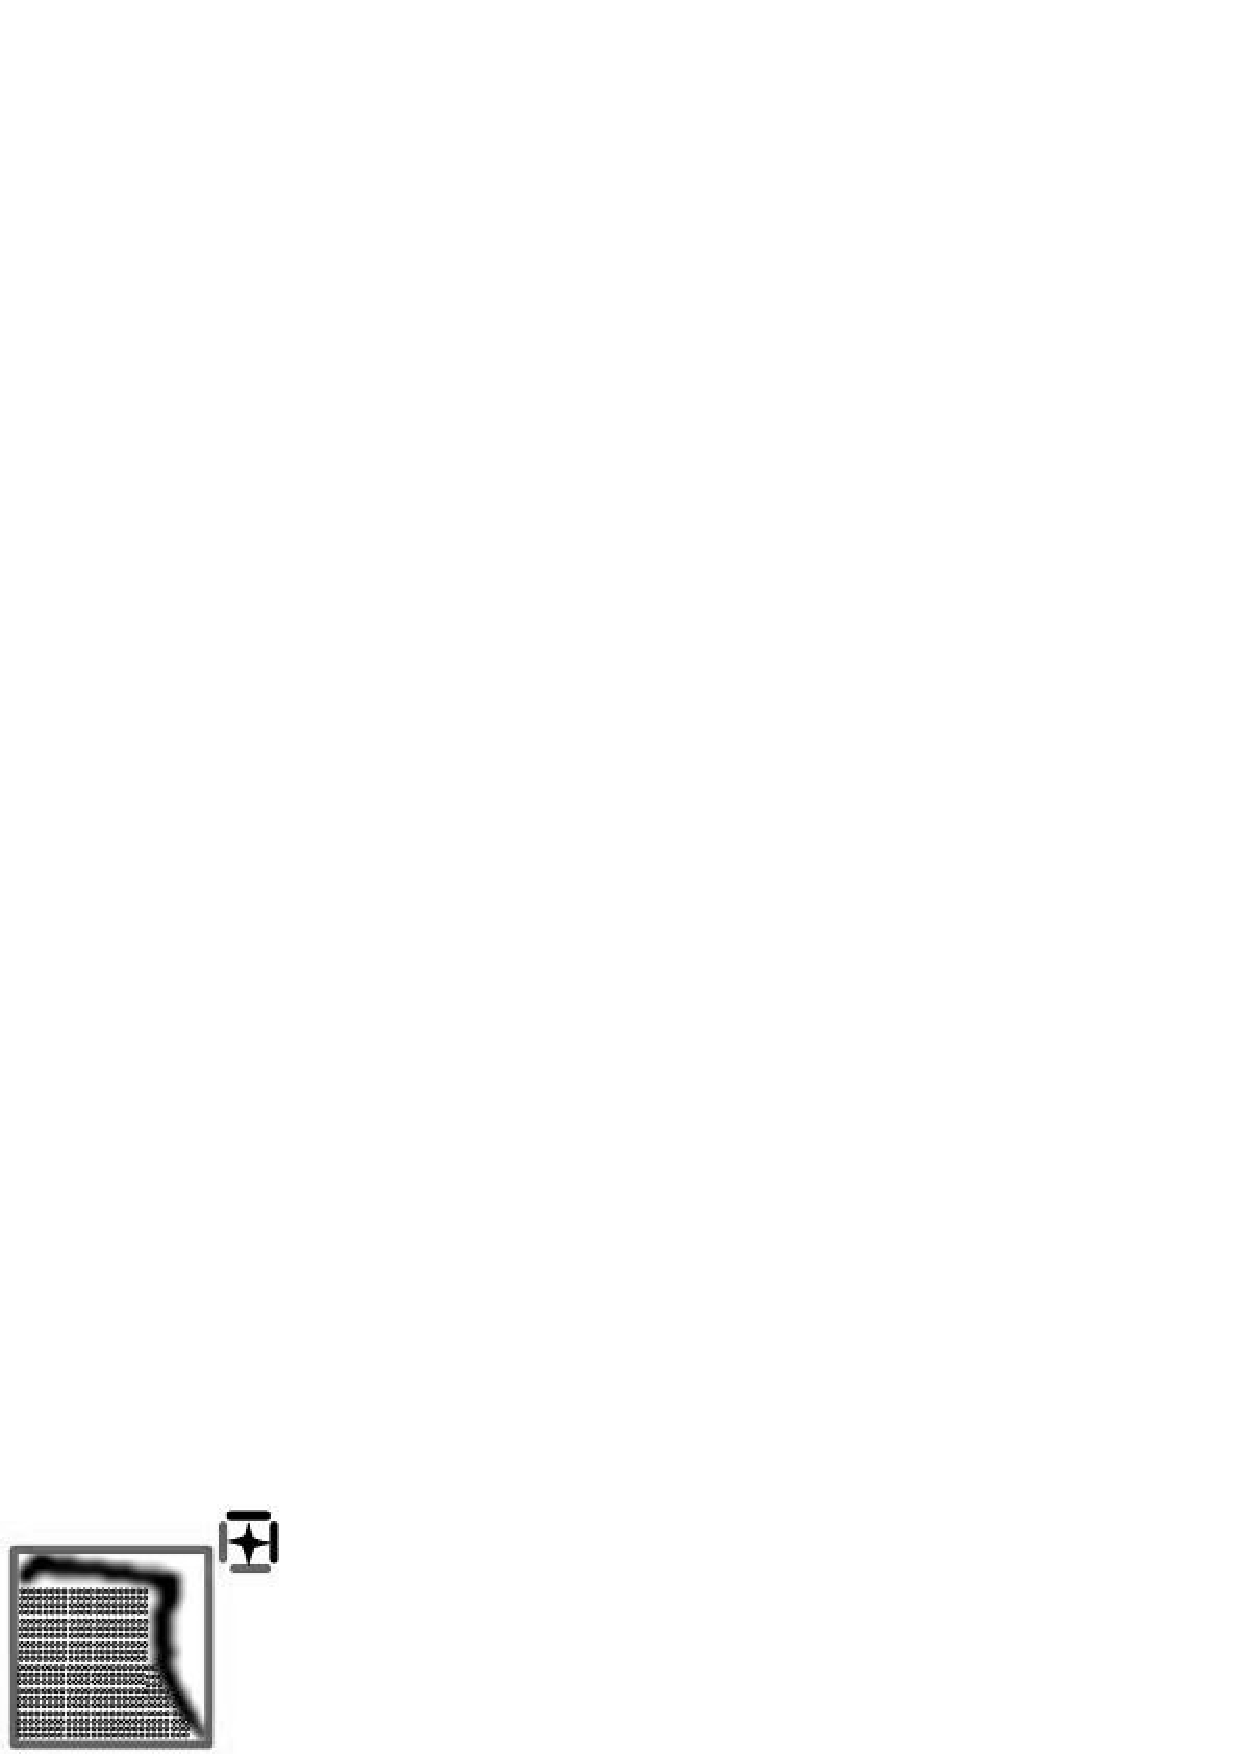
\includegraphics[width=0.15\textwidth]{figures/fig7.jpg}}
  \subfigure[Feature 'White\_3'.]{\label{fig:fig8}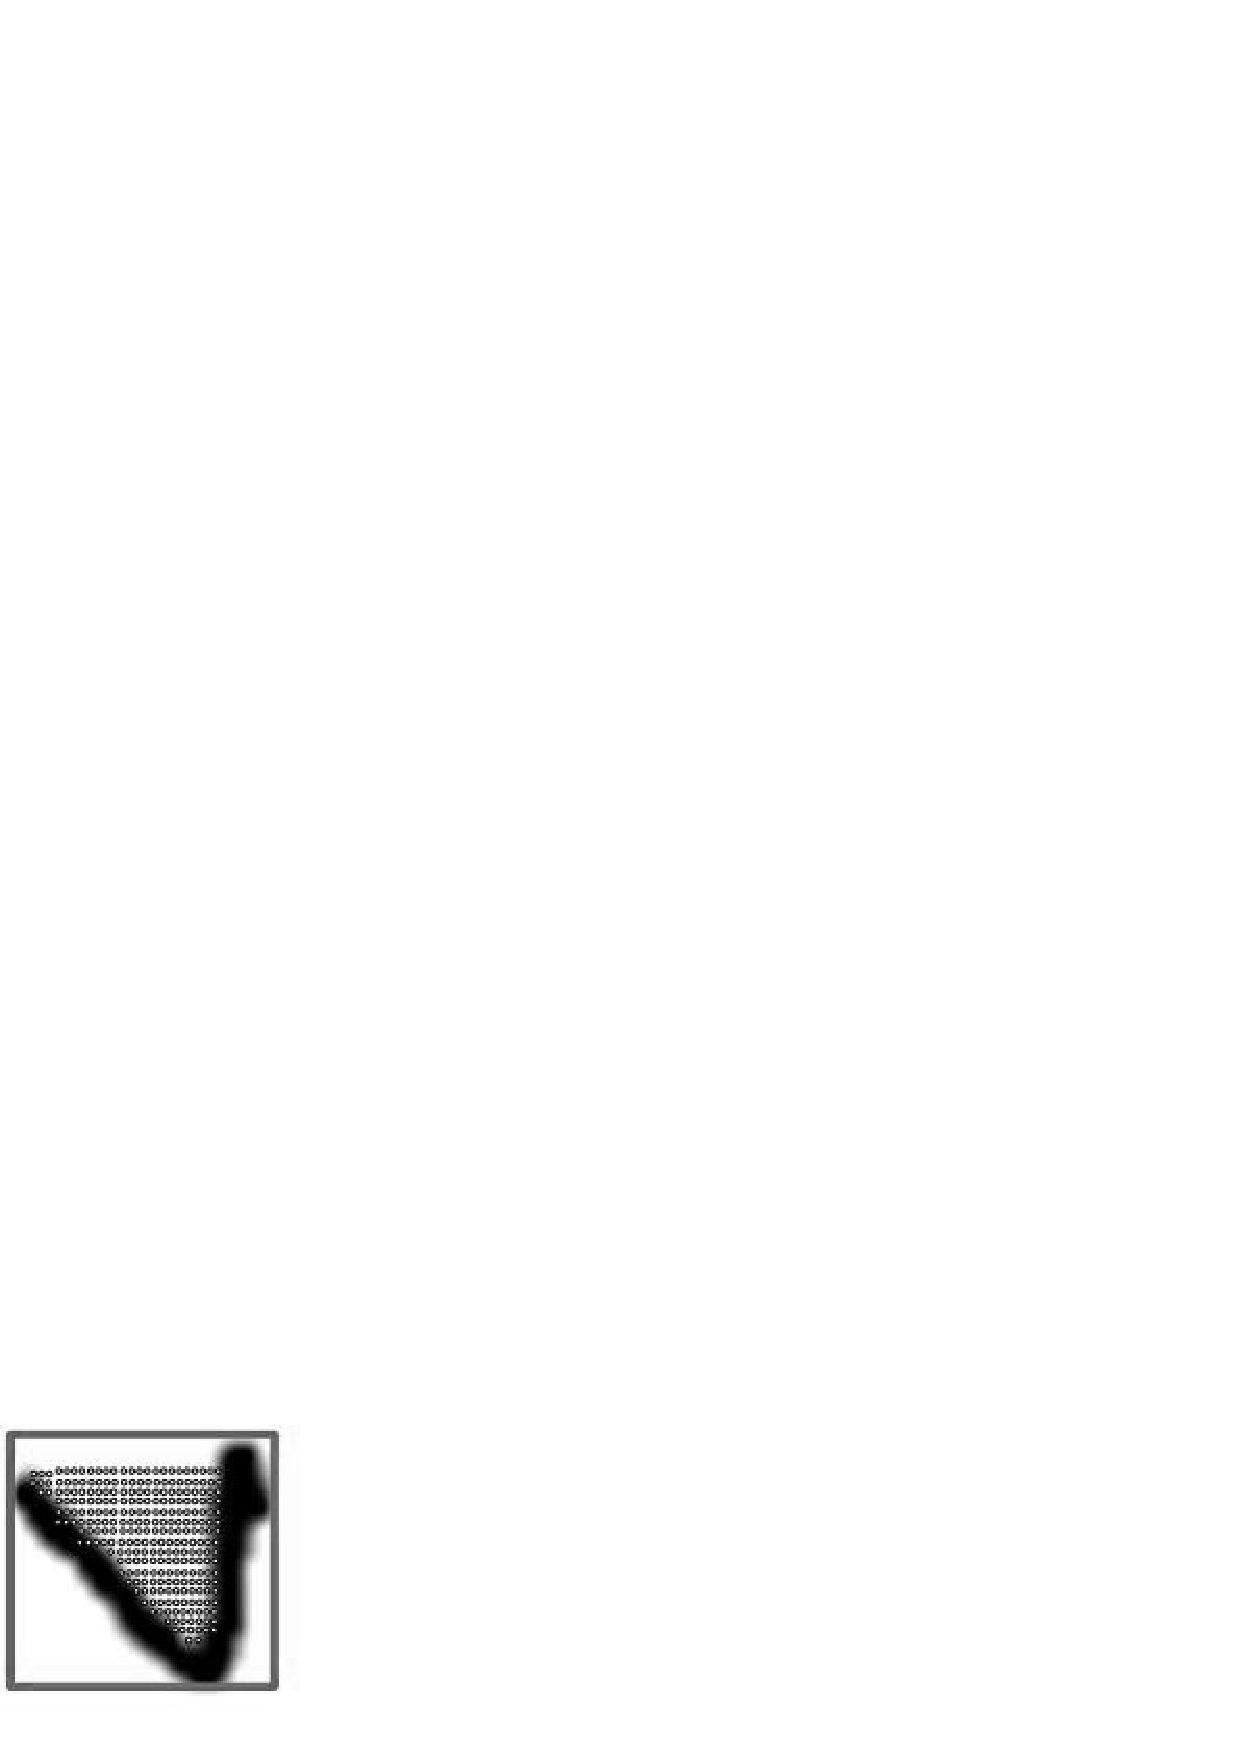
\includegraphics[width=0.15\textwidth]{figures/fig8.jpg}}
\end{center}
\caption{Feature 'White\_6' in Arabic digit 6 and Feature 'White\_3' in Arabic digit '7'.}
\end{figure} 

\textsl{Digit '6':} Arabic digit '6' is easily distinguishable by its white pixels surrounded by black pixels from the top and the right and by the left and bottom corners of the bounding box as shown in Figure \ref{fig:fig7}. The count of those white pixels is the discriminating feature of Arabic digit '6' and is denoted by 'White\_6'.

\textsl{Digit '7':} Arabic digit '7' is distinct by the number of white pixels surrounded by black pixels to their right and left and by the top corner of the bounding box from above as shown in Figure \ref{fig:fig8}. But this is the same feature 'White\_3' used before to distinguish digit '3' from digit '2'. However, the count of those pixels in digit '7' is usually larger than in digit '3'. Another distinguishing feature between digits '3' and '7' is the depth of those white pixels denoted by 'White\_3'. In digit '3', the 'White\_3' pixels usually exist in the upper half of the digit while in digit '7' they usually extend to the very bottom of the digit as clear in Figures \ref{fig:fig9}. The last row from the bottom that has 'White\_3' pixels is considered a feature and denoted 'White\_depth\_7'.
%Figure 9.  Feature 'White_depth\_7'.  
%\begin{figure}
% \begin{center}
% 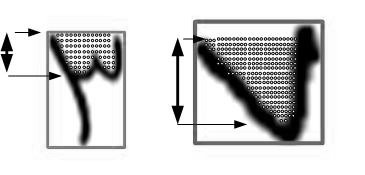
\includegraphics[width=0.2\textwidth]{figures/fig9.jpg}
%\end{center}
%\caption{Feature 'White\_depth\_7'.  }
%\label{fig:fig9}
%\end{figure} 

\begin{figure}
  \begin{center}
 \subfigure[Digit 3]{\label{fig:fig9a}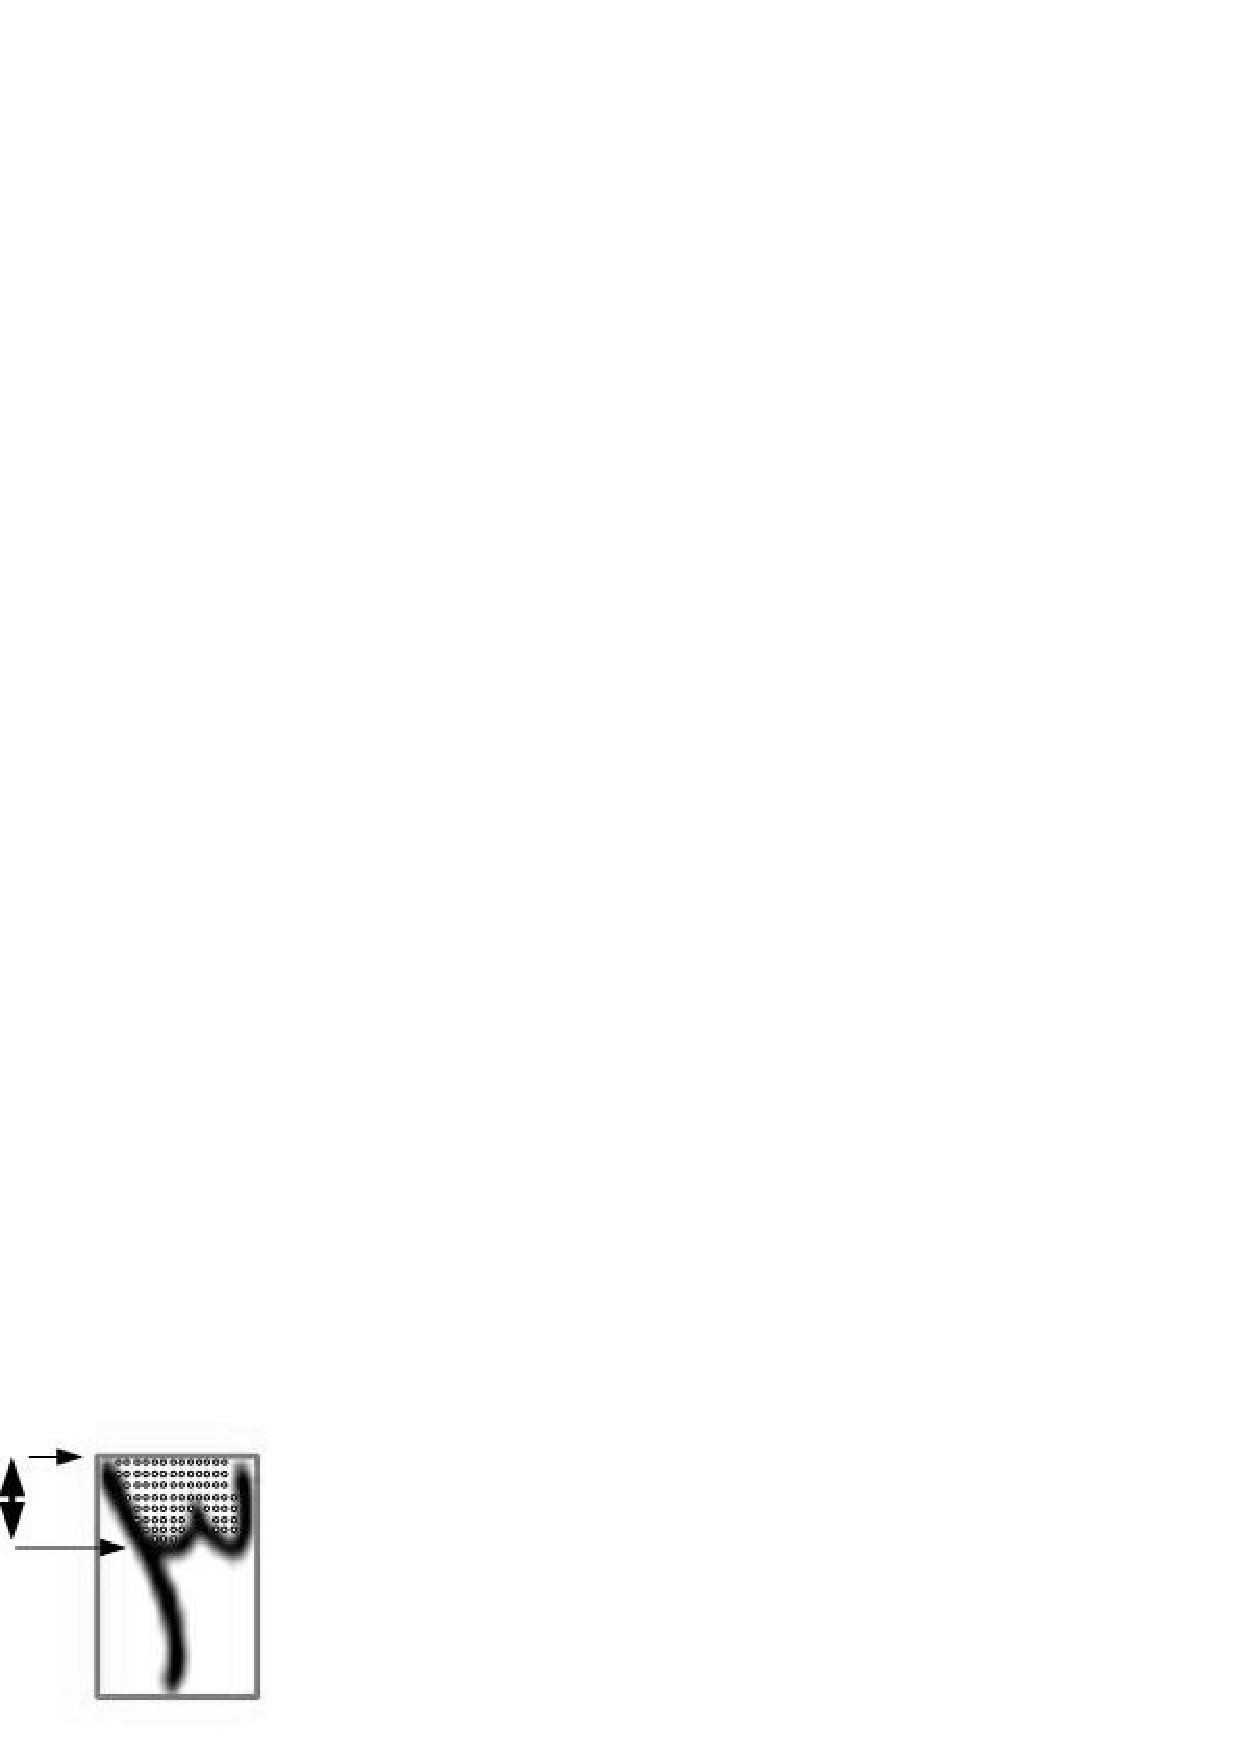
\includegraphics[width=0.1\textwidth]{figures/fig9a.jpg}}
  \subfigure[Digit 7]{\label{fig:fig9b}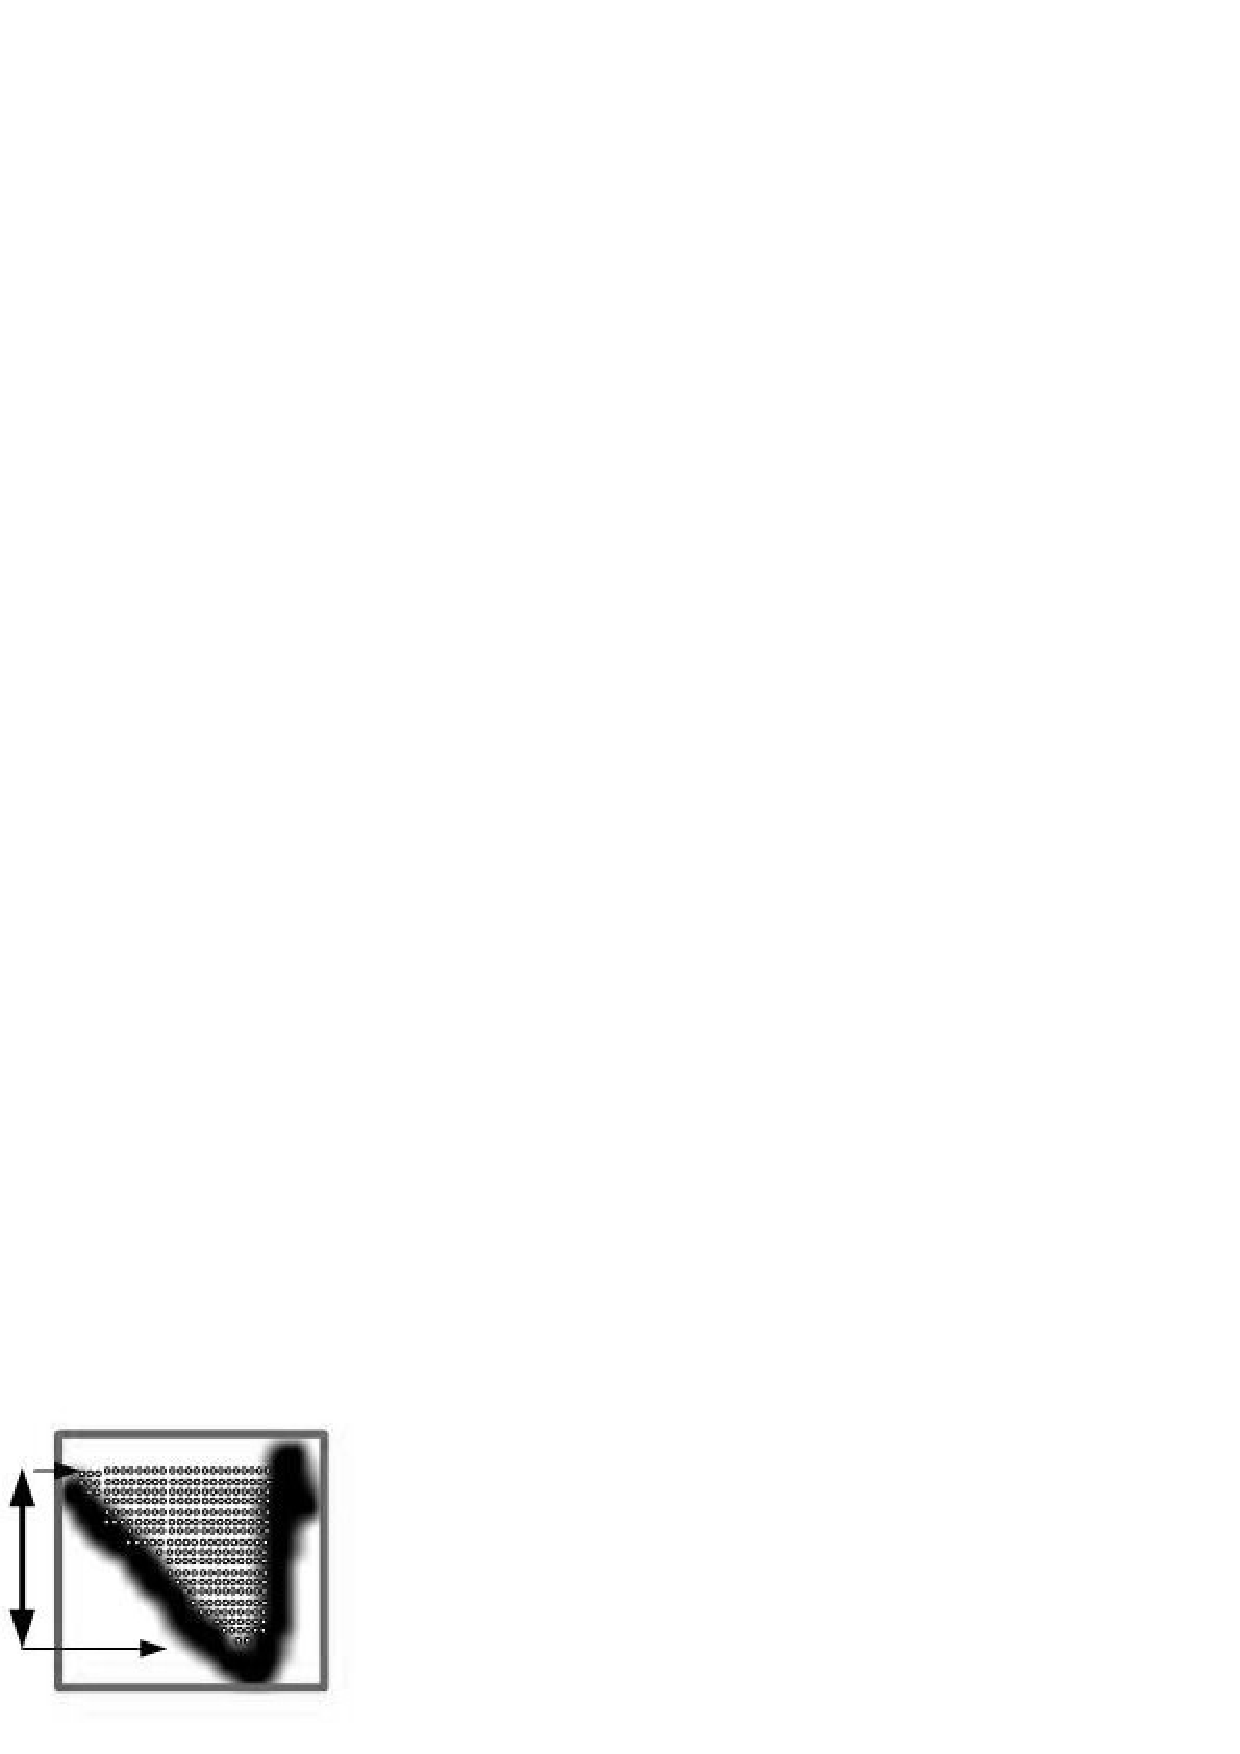
\includegraphics[width=0.1\textwidth]{figures/fig9b.jpg}}
  \end{center}
\caption{Feature 'White\_depth\_7'.  }
\label{fig:fig9}
\end{figure} 
%\subsection*{Digit '8'} 

\textsl{Digit '8':} Arabic digit '8' is distinct by the number of white pixels surrounded by black pixels to their right and left and by the bottom corner of the bounding box from below as shown in Figure \ref{fig:fig10}. The count of those white pixels is the discriminating feature of Arabic digit '8' and is denoted by 'White\_8'.

\begin{figure}
 \begin{center}
 \includegraphics[width=0.1\textwidth]{figures/fig10.jpg}
\end{center}
\caption{Feature 'White\_8'. }
\label{fig:fig10}
\end{figure} 
\textsl{Digit '9':} Arabic digit '9' can be distinguished by its white pixels surrounded by black pixels from the top and the right and by the left and bottom corners of the bounding box as shown in Figure \ref{fig:fig11}. Yet this is the same feature 'White\_6' used for Arabic digit '6' before. Other features are required to distinguish Arabic digit '9' from Arabic digit '6'. The number of white pixels surrounded by black pixels in all directions in the upper left half of the bounding box clearly distinguishes Arabic digit '9' from Arabic digit '6' as shown in Figure \ref{fig:fig11}. This feature is denoted by 'White\_9'. Another feature is the average height of the black pixels in the left half of the bounding box that is the distance between the first black pixel in one column and the last black pixel in the same column averaged over the columns of the left half of the bounding box as shown in Figure \ref{fig:fig12}. This feature is denoted by 'Black\_Height\_9'. 
\begin{figure}
 \begin{center}
  \subfigure['White\_6']{\label{fig:fig11a}\includegraphics[width=0.1\textwidth]{figures/fig11a.jpg}}
  \subfigure['White\_9']{\label{fig:fig11b}\includegraphics[width=0.1\textwidth]{figures/fig11b.jpg}}
 %\includegraphics[width=0.3\textwidth]{figures/fig11.jpg}
\end{center}
\caption{  Feature 'White\_6' and Feature 'White\_9'.  }
\label{fig:fig11}
\end{figure} 


%\begin{figure}
% \begin{center}
% \includegraphics[width=0.3\textwidth]{figures/fig11.jpg}
%\end{center}
%\caption{  Feature 'White\_6' and Feature 'White\_9'.  }
%\label{fig:fig11}
%\end{figure} 

\begin{figure}
 \begin{center}
 \subfigure[Digit 6]{\label{fig:fig12a}\includegraphics[width=0.15\textwidth]{figures/fig12a.jpg}}
  \subfigure[Digit 9]{\label{fig:fig12b}\includegraphics[width=0.15\textwidth]{figures/fig12b.jpg}}
 %\includegraphics[width=0.3\textwidth]{figures/fig12.jpg}
 % fig1.jpg.eps: 159x114 pixel, 72dpi, 5.61x4.02 cm, bb=0 0 159 114
\end{center}
\caption{ Feature 'Black\_Height\_9'.  }
\label{fig:fig12}
\end{figure} 
%\begin{figure}
% \begin{center}
% \includegraphics[width=0.3\textwidth]{figures/fig12.jpg}
% % fig1.jpg.eps: 159x114 pixel, 72dpi, 5.61x4.02 cm, bb=0 0 159 114
%\end{center}
%\caption{ Feature 'Black\_Height\_9'.  }
%\label{fig:fig12}
%\end{figure} 

\subsection{Validation}
The above 13 features are carefully chosen because of their intuitive discriminating ability for the ten numerals of the Arabic language. A linear SVM  classifier is used to train the featuers extracted from the MADBase training set. A validation set of 10,000 digits randomly selected from the training set has been used to check the effectiveness of this logical feature vector. The recognition rate of those 13 features was an impressive 98.22\% compared to 99\% achieved with a 200 gradient features on the same validation set. The fact that only 13 meaningful features can produce such high recognition rate encourages further search for more intuitive features imitating the process by which the human mind recognizes different digits. 

The process of further feature extraction has been continued on trial and error basis. That is, more intuitive features are extracted and every new feature is added to the original feature vector and then training and validation takes place. If the newly added feature improves the validation recognition results, it is appended to the feature vector or else it is discarded. The process of appending more features to the intuitive feature vector has been repeated until the validation recognition result exceeded that obtained by the 200 gradient features. An intuitive feature vector of 35 features has produced a recognition rate of 99.07\% outperforming the recognition results of the 200 gradient features vector. At that point, the process of appending more intuitive features has ended with an intuitive feature vector of 35 meaningful and easily extracted features that are able to compete with and outperform other well known feature vectors on the validation set. The first 13 features of the full feature vector have been explained above, the remaining 22 features are shown in Table \ref{tab:TheRemaining22FeaturesOfTheFullFeatureVector}. 

\begin{table*}
	\centering
		\caption{The remaining 22 features of the full feature vector}
	\label{tab:TheRemaining22FeaturesOfTheFullFeatureVector}
		\scalebox{0.85}{
		\begin{tabular}{|l|l|p{9.5cm}|l|}
		\hline 
	Num&	Feature & Description &	Distinguished digits  \\ \hline 
		14.	&'White\_Bottom' &
	Count of the white pixels contained between the bottom corner of the bounding box until black pixels are encountered.& 	6,8,9 versus rest	 \\ \hline 
15.&
	'White\_Right'&
	Count of the white pixels contained between the right corner of the bounding box until black pixels are encountered.& 	2,3,4 versus rest\\ \hline 
16.&	'White\_Top' &
	Count of the white pixels contained between the top corner of the bounding box until black pixels are encountered. &	3,7 versus rest\\ \hline 
17.&	'Max\_Left\_Transition' &
	Maximum distance between the column positions of the starting black pixels in any two consecutive rows inside the bounding box.& 	4,6,9 versus rest\\ \hline 
18.	&'Left\_Transition\_Location' &
	Row location of the above maximum left transition. &	6 versus 4,9\\ \hline 
19.	&'Max\_Right\_Transition'  &	Maximum distance between the column positions of the last black pixels in any two consecutive rows inside the bounding box.	&2,3,4 versus rest\\ \hline
20.	&'Right\_Transition\_Location'	& Row location of the above maximum right transition. &	2  versus 3\\ \hline 
21.	&'Sum\_Negative\_Transitions' &
	Number of rows in which the last black pixel is in a column to the left of the column of the last black pixel in the previous row. &	7 versus rest\\ \hline 
	22.	&'Sum\_Positive\_Transitions' &
	Number of rows in which the last black pixel is in a column to the right of the column of the last black pixel in the previous row.&	7 versus rest \\ \hline
23.&	'Sum\_Zero\_Transitions' &
	Number of rows in which the last black pixel is in the same column as the last black pixel in the previous row. 	&2,6,9 versus rest\\ \hline
24.&	'Sum\_Big\_Transitions' &
	Number of rows in which the last black pixel is in a column more than three pixels to the right of the column of the last black pixel in the previous row. &	4 versus rest\\ \hline
25.	&'Width\_Lower\_Half' &
	Number of rows in the lower half of the bounding box that are less than five black pixels. &	2,3,4,6,9 versus 5,7,8\\ \hline
26.&	'Small\_Width' &
	Number of rows in the bounding box that have black pixels spanning less than half the width of the bounding box. 	&2,3,4 versus rest\\ \hline
27.	&'Large\_Width' &
	Number of rows in the bounding box that have black pixels spanning more than one quarter of the width of the bounding box. 	&5,7,8 versus rest\\ \hline
28.	&'Black\_Top' &
	Count of the average number of black pixels in the top three rows of the bounding box. &	2 versus 3\\ \hline
29.&	'Black\_Bottom' &
	Count of the average number of black pixels in the bottom three rows of the bounding box. &	2 versus 4\\ \hline
30.	&'Black\_Left' 
	& Count of the average number of black pixels in the three columns at the left side of the bounding box. &	2 versus 6\\ \hline
31.&	'Black\_Right' &
	Count of the average number of black pixels in the three columns at the right side of the bounding box. &	2 versus 6\\ \hline
32.	& 'Top\_Black\_Turns ' &
	Count of the number of times the locations of the starting black pixels in the columns of the bounding box decrease then increase. &	3 versus 7\\ \hline
33.&	'Last\_Black\_Location' &
	The average row location of the last black pixels in the columns of the left half of the bounding box. 	& 6 versus 9\\ \hline
34.	&'Max\_Downward\_Transition'  &
	Maximum distance between the row positions of the last black pixels in any two consecutive columns inside the bounding box.& 	4,6,9 versus \\ \hline
35.&	'Downward\_Transition\_Location'&
	Column location of the above maximum downward transition. &	4 versus 9\\ \hline

	
		\end{tabular}
		}
\end{table*}

\section{Results}
\label{sec:section4}
The performance of the proposed feature vector with its 35 features has been tested on the test set of the MADBase. A linear SVM classifier has been used for that purpose. The proposed domain-specific intuitive feature vector resulted in a 99.25\% recognition accuracy outperforming all classification results obtained for the MADBase by a multitude of classifiers using various well known universal feature vectors as reported in \cite{IjdarSherifPaper}. The results of the various classifiers for the different feature sets are given in Table \ref{tab:AccuraciesOfClassifierFeaturesPairsOnMADBase}. It has to be noted here that the parameters of the classifiers used in Table \ref{tab:AccuraciesOfClassifierFeaturesPairsOnMADBase} such as number of hidden neurons of the neural network classifier, the C and and $\gamma$ of the RBF SVM, the C of the linear SVM, etc have been optimized using a validation set. 

\begin{table*}
	\centering
		\caption{Accuracies of classifier/features pairs on MADBase}
	\label{tab:AccuraciesOfClassifierFeaturesPairsOnMADBase}
	\scalebox{0.75}{
		\begin{tabular}{|l|c|c|c|c|c|c|c|c|c|c|}
		 \hline
  Feature	& KNN	& Parzen	& NN	&PCA + Quad	&Linear SVM	& SVM RBF 	&GC	&Fisher \\ \hline
	Gradient&	98.9	&98.92	&98.98	&99.11	&99.03&	99.18&	97.94	&98.27	\\ \hline	
	
	Kirsch &	98.14	&98.02	&98.5	&98.27&	98.82&	98.87&	97.25	&97.57\\ \hline
		Local Chain	&95.41&	94.32	&96.12	&96.46&	96	&97.08&	93.29&	95.72\\ \hline
Wavelet	&98.56	&98.34	&98.46	&98.03	&97.2&	98.85&	96.23	&95.53\\ \hline

		\end{tabular}
		}
\end{table*}

Comparing the 99.25\% accuracy achieved by the proposed feature set with the results shown in Table \ref{tab:AccuraciesOfClassifierFeaturesPairsOnMADBase} reveals the supremacy of the concept of feature extraction based on human intuition and the imitation of how the human mind discriminates between the different digits. It goes without saying that the proposed 35 features have their own limitations and there are still 75 digits in the test set of 10000 digits that could not be recognized by them using the linear SVM classifier. 

It should be noted that the performance of the smaller feature vector of the 13 intuitive features described in Section 3 has achieved 98.26\% accuracy on the MADBase test set using linear SVM. Comparing this result with those in Table \ref{tab:AccuraciesOfClassifierFeaturesPairsOnMADBase} proves that a small feature vector of merely 13 features can outperform other well known feature sets such as the chain code features and the wavelet features for the same linear SVM classifier. This means that some few basic and intuitive features can achieve remarkable success in recognizing at least the easily recognizable digits in the test set. More difficult test digits still require more and more features to be added to the feature vector to improve the recognition rate on the test set.  

It is important to note that the significance of the concept of handpicked features proposed in this paper goes beyond improving the recognition accuracy. The proposed feature vector is much smaller and simpler than the universal feature sets known in the literature. The computational complexity involved with extracting only 35 features is certainly less than that of extracting hundreds of features. More importantly, the proposed features are all simple to extract because they are usually simple counts of distances or counts of white or black pixels with certain characteristics existing within the bounding box. No special computations like calculating gradients or detecting edges are involved. The actual feature extraction time of the proposed feature vector, for the entire MADBase test set, has been measured and compared with the time taken for the feature extraction of the feature sets used in Table \ref{tab:AccuraciesOfClassifierFeaturesPairsOnMADBase}. The results are given in Table \ref{tab:FeatureExtractionTimeOfVariousFeatureSets}. All the experiments have been implemented on a PC with 1.6GHz Intel processor and 1GB RAM using MATLAB 7.5.

\begin{table}
\caption{ Feature extraction time of various feature sets}
	\label{tab:FeatureExtractionTimeOfVariousFeatureSets}
	\centering
	\scalebox{0.7}{
		\begin{tabular}{|c|c|}
			\hline 
			Feature &	Time \\ \hline
Domain-specific features &	6.6015\\ \hline
Kirsch	&9.72525\\ \hline
Gradient&	107.70325\\ \hline
Wavelet	&92.04\\ \hline
Local Chain	&130.57\\ \hline
		
		\end{tabular}
		}
\end{table}

\section{Concluding Remarks}
\label{sec:section5}
In this paper, it is argued that a carefully chosen feature vector representing the peculiarities of every individual digit of the Arabic language can outperform much larger general purpose feature vectors in the two important requirements of any successful recognition system: accuracy and speed. The fact that only 35 handpicked features can surpass well known universal feature sets including the powerful gradient feature vector with 200 features proves that domain-specific features should receive more attention by researchers. It should be noted that the feature set of 35 domain-specific features proposed in this paper is not necessarily the best domain-specific feature set for the problem of Arabic handwritten digit recognition. That is, there could be other domain-specific features that perform better than the feature set presented here or there could be other features if added to the proposed 35 features would improve the recognition results further. The main theme of this paper is neither the feature set that produces the highest recognition rate nor the most compact feature set but rather the concept that a feature set which is problem-specific and based on the way humans visually distinguish the classes at hand can outperform universal feature sets in both accuracy and speed. But the extraction of the best possible domain-specific feature set is an open question and requires further research.

In fact, the success of the problem-specific feature extraction approach with Arabic handwritten digits should motivate further research in various directions. The same approach can be applied to other languages and other character recognition problems. The automation of the generation of problem-specific features that match the human visual understanding of the classes at hand is another avenue for future research. Hybrid feature extraction that involves both universal and problem-specific features is a different research direction. The speed of feature extraction of some domain-specific features makes them good candidates to be used in the early stages of classification cascades where the concern is speeding up the classification process without sacrificing the classification accuracy \cite{optimumPaper,GreedyPaper}. One-versus-one problem-specific feature extraction where the features are extracted to distinguish every individual pair of classes from one another may enhance the overall recognition accuracy.
\bibliographystyle{unsrt}
%\bibliographystyle{latex8} 
\bibliography{../../PaperDBase/library}
\end{document}
